\documentclass[letterpaper,8pt]{article}  % "extarticle" gives more global font size options. use 8pt with Montserrat and 10pt with EBGaramond
\usepackage{import}
\usepackage{local}
\usepackage{amsmath}
\usepackage{subcaption}
\usepackage{float}
\usepackage{sidecap}
\sidecaptionvpos{figure}{m}
\usepackage[left=.95in,top=.65in,bottom=.75in,right=.85in]{geometry}
\usepackage{lipsum} % to generate text

\title{(Temporary...) Overlooked model uncertainties may misinform forest management strategies}

\author{%
\textbf{Victor Van der Meersch\textcolor{Accent}{\textsuperscript{1*}}, %
Isabelle Chuine\textcolor{Accent}{\textsuperscript{1}} %
}\\
\begin{small}\textcolor{Accent}{\textsuperscript{1}}CEFE, CNRS, Univ. Montpellier - 34000 Montpellier, France \\ 
\textcolor{Accent}{\textsuperscript{*}}Correspondence: \textcolor{Accent}{victor.vandermeersch@cefe.cnrs.fr} \\ \end{small}
}


\date{}
\begin{document}

\maketitle

\section*{Abstract}

\begin{doublespacing}
\begin{linenumbers}

Climate change poses significant challenges to forest management in Europe, where rising temperatures and increased frequency of extreme weather events threaten forest health and productivity. Thus, policy makers and forest managers urgently need robust projections of the suitability of future climatic conditions for5 forest tree species to guide conservation efforts, forest management strategies and make informed decisions. Previous studies, which aimed at providing such projections, mostly made use of a single type of model to do so (correlative models) and failed evaluating the uncertainties associated with the model projections. Here, we simulated the distribution of six European tree species over the 21\textsuperscript{st} century, using various correlative and process-explicit models and the most recent climatic projections (SSP2 and SSP5 scenarios). We examined several versions of the models differing by their complexity and calibration methods in order to identify and quantify the different sources of uncertainty in their projections. We find (i) that the use of occurrence data to calibrate models, whether correlative or process-explicit, consistently leads to more pessimistic predictions, and (ii) that using different modelling approaches together allow to assess more rigorously projection uncertainties. Evaluating and communicating the degree of uncertainty enhances the credibility of species distribution models, and contributes to a better adaptation to the impacts of climate change on forest ecosystems.

\rmfamily


\subsection{Introduction}

% Current state 
Forests are increasingly under pressure from climate change. In Europe, where temperatures are rising twice as fast as the global average \citep{CCCS2024}, unprecedented pulses of tree mortality were reported in the last decade \citep{Senf2020}. These damages are observed not only in populations living at the margins of their climatic range, but also in those living in the core of their range. Some European forests have even become net CO2 sources recently  in some areas \citep{Hadden2016, Karelin2021}, due to decreased growth \citep{Hadden2016, Woude2023}, increased burned areas \citep{Carnicer2022, Kelly2024}, and increased dieback driven by increased drought frequency and intensity and increased vulnerability to pest attacks \citep{Karelin2021, Cienciala2024, Latifovic2024}.

% Need to act
Forests have nevertheless a major role to play in mitigating climate change and achieving carbon neutrality \citep{Korosuo2023, Hyyrynen2023}. Forests managers are facing unprecedented short-term and long-term challenges, as they need to address current dieback issues while promoting forest adaptation to climate change. These decisions have to be made in a context of high uncertainty, because of the lack of data and knowledge about the effects of climate change, interacting with various forest management strategies.

% But to take decisions, we need... model projections
While long-term experiments yield unique insights into biological processes at stake, predictive ecological models are essential to complement and extend them by examining the drivers operating at large spatiotemporal scales \citep{Levins1993, Mitchell2006}. Some of these models aimed at identifying, at the regional or continental scale, which species will be able to grow in future climatic conditions. Most studies project pronounced species range shifts and forest composition changes in Europe. Deciduous late-successional species, mostly oaks (\emph{Quercus robur} L., \emph{Quercus petraea} (Matt.) Liebl.) and beech (\emph{Fagus sylvatica} L.), are expected to expand their range towards North-eastern Europe and decline in France \citep{Hickler2012, Hanewinkel2013, Saltre2015, Schueler2014, Dyderski2018, Takolander2019, Wessely2024}. Areas suitable for Mediterranean oak forests, including for evergreen oak, should increase \citep{Ohlemueller2006, Hanewinkel2013, Takolander2019}. On the contrary, coniferous trees, such as spruce (\emph{Picea abies} L.) or pine (\emph{Pinus sylvestris} L.), may loose large portions of their current range \citep{Hanewinkel2013, Schueler2014, Wessely2024}. These climate-induced species shifts are predicted to have major impacts on timber production and forest economic sector \citep{Hanewinkel2013, Wessely2024}. 

% But the future is uncertain, and so are our projections
However, there is often considerable uncertainty associated with the future trajectory of ecosystems. Model projections are subject to many sources of uncertainty, whether they are correlative species distribution models (CSDMs) or process-explicit models (PEMs). Most studies have relied on correlative approaches, and, when the uncertainties were addressed (which is not at all systematic; \citealp{Simmonds2024}), they primarily focused on three sources of errors: the data quality used for model fitting \citep{Chen2013, BarbetMassin2010, Duputie2014, Faurby2018}, the variation among climate change projections \citep{Beaumont2007, DinizFilho2009, Thuiller2019}, and the variation among modeling method \citep{Pearson2006, DinizFilho2009, Thuiller2019}. The latter often only corresponds to the fitting algorithm (GLM, GAM, Random Forest...). Even though the differences between these algorithms can be significant, previous studies are still far from encompassing the diversity of modeling approaches that exist \citep{Dormann2012}. They thus ignore a large part of the methodological uncertainty of the projections. This is a major shortcoming, especially since process-explicit models might be more robust under novel climatic conditions (\citealp{VanderMeersch2024}; \hyperref[chapter2]{Chapter 2}).

% Current knowledge about CSDM/PBM projection differences
The handful of studies that have compared CSDMs with PEMs have shown that their projections indeed significantly diverge in future climatic conditions \citep{Morin2009, Keenan2011a, Cheaib2012, Takolander2019}, and PEM projections tend to be more nuanced. These studies have provided some essential insights, though they were limited to a qualitative comparison of projections over a limited area and did not account for climatic uncertainties (i.e. they used a single climate model). Today, it is nevertheless essential to quantitatively understand how the different approaches of species distribution models influence the uncertainty of projections, considering the interaction with the climate, and how these uncertainties will evolve over time.

% Why a step forward is urgently needed to support decision-making
Understanding where do the uncertainties originate and  and how they relate to each other is indeed a critical challenge. From the modeler point of view, it is obviously crucial to identify opportunities for model developments \citep{Petchey2015}. But it has broader implications beyond the scientific community, to address policy-relevant questions \citep{Urban2016}. Clarifying and quantifying the many uncertainties that the different actors will face in the 21\textsuperscript{st} century supports the development of robust and sustainable forest management practices that can accommodate a range of possible future scenarios \citep{IPCC2021}. In particular, it helps identify how serious the risk is for the forest considered, and if any action is required. Forest managers need to know whether the current species will be able to tolerate future climate conditions, whether they can rely on its natural regeneration, or whether they should capitalize on new species opportunities. It is not reasonable to ignore these uncertainties or to consider only a portion (e.g. omitting model methodological uncertainty) if we aim to secure the capacity of Europe’s forests to continue providing ecosystem services. 

% What we've done
To capture the full breadth of uncertainties that are relevant to assess how climate change will affect forests across Europe,
we simulated the future distribution of six tree species (\emph{Abies alba} Mill., \emph{Fagus sylvatica} L., \emph{Quercus petraea} (Matt.) Liebl., \emph{Quercus robur} L., \emph{Quercus pubescens} Willd. and \emph{Quercus ilex} L.) with different modeling approaches, using 10 different climate projections (5 global climate models and 2 socioeconomic scenarios) from the CMIP6 dataset \citep{Noel2022}. We then used an ANOVA-based variance decomposition to identify the different sources of uncertainty and quantify their relative contribution to the total projection uncertainty.

\clearpage

\subsection{Methods}

\subsubsection{Species distribution models}

We sought to encompass the greatest diversity of species distribution modeling (SDM) approaches by including three different approaches, along the correlative–process spectrum \citep{Dormann2012}: correlative models (CSDMs), process-explicit models (PEMs) and fitted PEMs (hybrid approach between CSDM and PEM).

For the correlative approach, we selected five well-established models following the performance comparison by \cite{Valavi2022}: GLM with lasso regularization, GAM, BRT, MaxEnt and down-sampled Random Forest. We selected a set of uncorrelated climate predictors, based on their implicit relevance for tree species: minimum temperature of the coldest month (representing frost tolerance), total precipitation (representing available water), GDD5 (growing degree days \textgreater5°C) between April and September (representing available thermal energy for vegetation growth and fruit maturation), and water balance between June and July (difference of precipitation and evapotranspiration, representing summer drought tolerance). We also included two soil covariates (pH and Water Holding Capacity). We calibrated the models using species occurrences from the dataset assembled in \cite{VanderMeersch2023}, mostly based on EU-Forest inventory data \citep{Mauri2017}, and 50,000 background points (to properly represent the full range of environmental conditions across Europe, \citealp{Valavi2022}). For each model and each species, we ran a fivefold environmental cross-validation to estimate model performance in novel extrapolation conditions \citep{Roberts2017}. We then used all the available training data to calibrate the models in order to favour final prediction quality \citep{Roberts2017}.

For the process-explicit approach, we used the model PHENOFIT. It assesses the fitness of an adult tree by simulating the precise phenology (leaf unfolding, flowering, fruit maturation, leaf senescence), and damages caused by abiotic stress (frost, drought) relatively to the development stages of the different organs. The parameters of PHENOFIT are either calibrated with direct measurements, literature data, or inferred  using observations of the processes modelled (e.g. species-specific phenological dates to calibrate phenological subcomponents). Its calibration thus does not involve species occurrence data. PHENOFIT requires daily climate variables, as well as the soil water holding capacity. The model has been validated for several North American and European species, either in historical or Holocene climatic conditions \citep{Morin2007, Saltre2013, Duputie2015, Gauzere2020, VanderMeersch2024}. This modeling approach will be referred to as \emph{expert} PEM in the following.

We also included a fitted PEM, somewhere in the middle of the correlation–process continuum \citep{Dormann2012}. To this aim, we calibrated PHENOFIT using species occurrence data as CSDM do, with the constraints of the model's process-explicit structure. We optimized the parameters of the model using the covariance matrix adaptation evolution strategy (CMA-ES, \citep{Hansen2001}), on a multicore cluster, following \citet{VanderMeersch2023}. To reduce the computational cost of this inverse calibration, we calibrated the model with subsets of 2000 points (1000 presences and 1000 absences), from the same dataset as correlative models (see above). We calibrated 10 times each species parameter set, with five repetitions on two random subsets of presences/pseudo-absences (except for beech, for which we ran 10 repetitions on 10 subsets).

The three modeling approaches output a variable between 0 and 1, indicating how well the climate is suitable for the species. This suitability index can be converted into a binary predictor, with a threshold that maximizes the true skill statistic (TSS, calculated from a confusion matrix). 

The robustness of these three different approaches was assessed by hindcasting the range shifts of five forest tree species across Europe over the last 12,000 years (\citealp{VanderMeersch2024}; \hyperref[chapter2]{Chapter 2}). The results indicated that the transferability of PEMs (either expert or fitted) was higher in climates that were significantly different from the historical period.

Finally, for beech only, we also included a \emph{partially} fitted PEM. It was calibrated in the same way as the fitted PEM, but we optimized only some critical parameters that were identified as responsible for errors in the expert PEM simulations (\hyperref[chapter3]{Chapter 3}). Other parameters were fixed at the expert values. Note thas this partially fitted PEM was not included in the uncertainty partitioning (see below).

\subsubsection{Environmental data}

CSDMs and fitted PEMs were calibrated with historical climatic conditions (1970-2000) from ERA5-Land dataset at a 0.1\degree resolution \citep{MunozSabater2021}. Soil data were extracted from EU-SoilHydroGrids \citep{Toth2017} and SoilGrids \citep{Hengl2017} databases.

Future simulations were run with the last Coupled Model Intercomparison Project Phase 6 (CMIP6) climate  projections, for 5 global climate models (GCMs) and 2 shared socio-economic pathways (SSPs). 
Model projections were downscaled to a 0.1° resolution with a statistical trend-preserving method (the cumulative distribution function transform), using the ERA5-Land reanalysis as a reference observational dataset between 1981 and 2010 \citep{Noel2022}. The five GCMs were GFDL-ESM4 \citep{Dunne2020}, IPSL-CM6A-LR \citep{Lurton2020}, MPI-ESM1-2-HR \citep{Mueller2018}, MRI-ESM2-0 \citep{Yukimoto2019} and UKESM1-0-LL \citep{Sellar2020}. They are considered as good representatives of the full CMIP6 ensemble \citep{Noel2022}. We selected scenarios SSP2-4.5 and SSP5-8.5, because the projected total cumulative CO2 emissions according to two International Energy Agency scenarios fall between these two SSPs \citep{Schwalm2020}. However, recent studies argue that SSP5-8.5 is unlikely \citep{Hausfather2020}, and current policies may rather lead to greenhouse gas emissions similar to those in SSP2-4.5 \citep{Gillett2024}. Accordingly, when only one SSP was considered, we chose SSP2-4.5 (\Cref{fig:cascade,,fig:fagus}). In cases where both SSPs were used (\Cref{fig:anovaecoregions,,fig:anova2090,,fig:anovawithinspecies}), note that the uncertainty related to the 5 GCMs used is consistently higher than the SSP uncertainty.

For PHENOFIT, we extracted the following daily climate variables: minimum, mean and maximum daily temperatures, daily precipitation, daily global radiationdaily mean wind speed and daily relative humidity. We then computed the daily potential evapotranspiration with Penman–Monteith equation (FAO standard, \citealp{Allen1998}). Finally, for the correlative models, we used these daily variables to calculate the 4 climate predictors described above.  Soil conditions (needed both for correlative and process-explicit models) were held constant throughout the simulations.

\subsubsection{Uncertainty partitioning}

Our approach was inspired by the partitioning of uncertainties in climate projections initially developed by Hawkins and Sutton \citep{Hawkins2009, Hawkins2011}, which was subsequently enhanced with additional methodologies \citep[e.g.][]{Yip2011, Lafferty2023}. 
Rather than using a simple variance decomposition approach, we perform an ANOVA-based variance decomposition to also estimate the importance of the two-way interaction effects. All analyses were performed in R \citep{RCT2024}.

Across all species, we partitioned three sources of uncertainty: the climate projection uncertainty related to the different GCMs, SSPs, and their interaction, the species distribution modeling uncertainty related to the differents SDMs, and the species uncertainty related to the different species specific responses to climate change. We also considered the interactions between SDMs and climate projections (GCMs and SSPs), between SDMs and species, and between species and climate projections (\Cref{fig:anovaecoregions}). For each year, the suitability of a cell was considered as a 21-year moving average suitability (e.g. 2040-2060 for the year 2050). We then computed the difference of suitability with the historical suitability (computed for each GCM on the period 1970-2000). For each GCM and each SSP, when multiple SDM projections were simulated within the same SDM approach (e.g. multiple inverse calibrations), we kept one ensemble per approach. For each year $t$, we then applied a linear ANOVA to calculate the sums of squares attributable to each uncertainty source:
\begin{multline*}
{SS}_{tot} = {SS}_{GCM} + {SS}_{SSP} + {SS}_{GCM:SSP} + {SS}_{SDM} + {SS}_{SDM:GCM} + {SS}_{SDM:SSP}\\+ {SS}_{species} + {SS}_{species:GCM} + {SS}_{species:SSP} + {SS}_{species:SDM} + {SS}_{residuals}
\end{multline*}

We then computed 90\% uncertainty ranges additively and symmetrically around the mean projection (across all GCMs, SSPs, SDMs and species), e.g. for SDM uncertainty: $\pm1.645*\sigma*\frac{{SS}_{SDM}}{{SS}_{tot}}$ (\Cref{fig:anovaecoregions}).
Finally, we also partitioned the variance within each species. This implies applying the same ANOVA, but on species-level predictions, and thus dropping the species-related coefficients (\Cref{fig:anovawithinspecies}).

\subsection{Results}

The magnitude of uncertainties varied across ecoregions (\Cref{fig:anovaecoregions}). In most Europe (Atlantic, Continental and Boreal), the 90\% confidence interval encompassed a wide range of projected change in suitability (relative to the 1970-2000 reference period), and uncertainties increased significantly the further we get into the future. In Mediterranean and Alpine ecoregions, the confidence interval was narrower and it increased much less with time (\Cref{fig:anovaecoregions}). Despite these large uncertainties, trends could still be observed across Europe, along a Southwest to Northeast gradient (\Cref{fig:anova2090A}). For the 6 species considered here, the average projected suitability decreased in the Mediterranean Basin while it increased in the Boreal region as it could have been expected (\Cref{fig:anovaecoregions,,fig:anova2090A}). However, for the continental ecoregion, the trend was less clear and models showed the lowest agreement (\Cref{fig:anova2090A}).

\begin{figure}[H]
\vspace*{0cm}
\centering
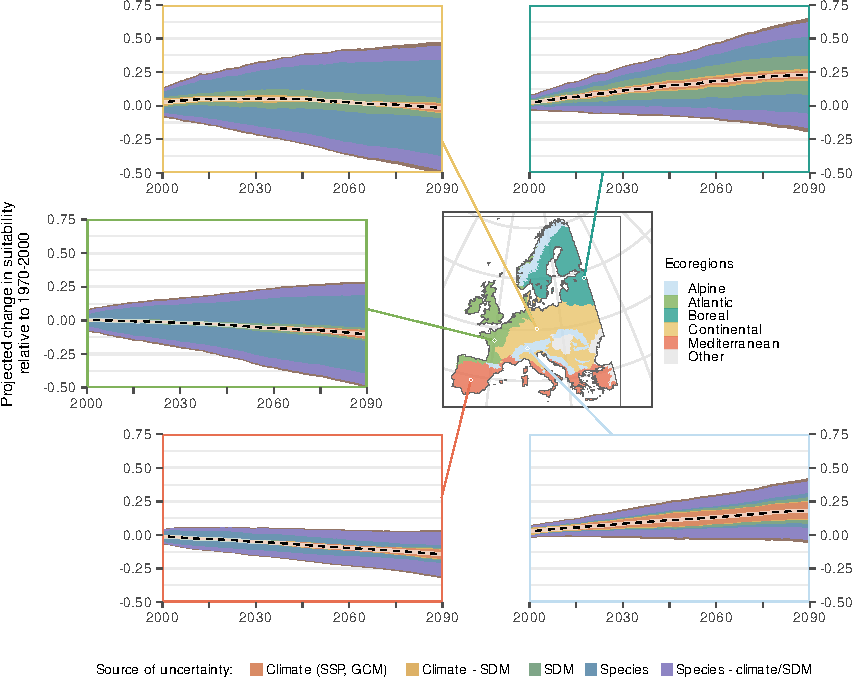
\includegraphics{figures/anova_across_species_byecoregion-1.pdf}
\caption{\textbf{Evolution of climatic suitability change and variance partitioning across Europe's ecoregions.} An ANOVA-based variance decomposition was performed to distinguish between 5 main uncertainty sources: (i) the future climate projections (GCM, SSP, and their interactions), (ii) the interactions between SDM approach and climate projections (both GCMs and SSPs), (iii) the SDM approach, (iv) the tree species, and (v) the interactions between species and both climate projections and SDM approaches. The dotted line represents the mean projection, across all GCMs, SSPs, SDMs and species. 90\% uncertainty ranges were calculated additively and symmetrically around the mean.}
\label{fig:anovaecoregions}
\vspace*{0cm}
\end{figure}

The effects of the climate projections, the species  and the modeling approach differed with respect to the ecoregion considered. Climate projection was the main source of uncertainty in the Alpine ecoregion, explaining 44\% of total uncertainty in 2090 (\Cref{fig:anovaecoregions,,fig:anova2090B,,fig:anova2090C}), while in the Atlantic and Continental ecoregions diferences between species responses was the main source of uncertainty (respectively 56.6\% and 42.4\% in 2090; \Cref{fig:anova2090B,,fig:anova2090C}). Interestingly, modelling approach was respectively the first and the second source of uncertainty in the Boreal (33.7\%) and the Continental (29.4\%) ecoregions (\Cref{fig:anova2090C,,app:frac}), which represent 58.6\% of Europe total forest cover (\Cref{tab:forest}).

Two-way interactions between species and both climate projections and modeling approaches also represent a significant contribution to the total uncertainty (\Cref{fig:anovaecoregions}). In 2090, they represent the major source of uncertainty in the Mediterranean ecoregion  (50.1\%; \Cref{fig:anova2090B,,fig:anova2090C}), and explain between 15.1\% and 20.7\% of the total uncertainty of the four other ecoregions. This stresses the importance of using ANOVAs to properly account for these interactions. In particular, the interaction between the species considered and the modelling approach is by far the most important factor (\Cref{app:specinter}), and reveals contrasted trends depending on the model and the species considered (\Cref{app:spectrend}). 

\begin{figure}[hp]
\centering
\begin{subcaptiongroup}
\phantomcaption\label{fig:anova2090A} 
\phantomcaption\label{fig:anova2090B}
\phantomcaption\label{fig:anova2090C}
\end{subcaptiongroup}
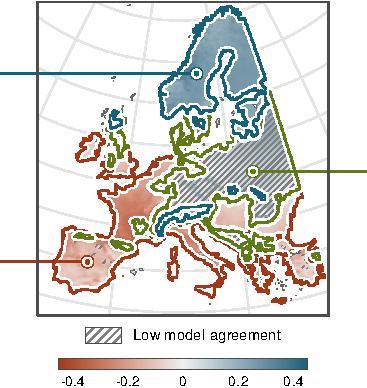
\includegraphics{figures/anova_across_species_bycell-1.pdf}
\caption{\textbf{Projections of climatic suitability change and main source of uncertainty in 2090.} (a) Overall change in fitness between the projection period 2080-2010 and the reference period 1970-2000, across all GCMs, SSPs, SDM approaches and species. Hashed shading reflects area where the three approaches of SDMs did not agree in the sign of suitability change. (b) Main source of uncertainty over the 2080-2100 period, according to a cell-based ANOVA partitioning. (c) Variance partitioning across Europe's ecoregions, for the 2080-2100 period. The black line represents the mean projection, across all GCMs, SSPs, SDMs and species. 90\% uncertainty ranges were calculated additively and symmetrically around the mean.}
\label{fig:anova2090}
\end{figure}

At the species level, most uncertainty arises from the discrepancy between the projections of the different SDMs (\Cref{fig:anovawithinspecies}). Except for the Alpine region, SDM approach consistently represents the major source of uncertainty for the four other ecoregions (between 54.2\% and 64.8\%). For example, in the Continental ecoregion, differences across models account for 73.7\% of the total uncertainty of beech future suitability, despite being within the core of its present distribution. Similarly, SDM is the main source of uncertainty for sessile and pedunculate oaks (respectively 57\% and 76.8\%, \Cref{fig:anovawithinspecies}). In Atlantic and Continental regions, the differences between species are strong: all models agreee with a lower suitability for fir and a higher suitability for holm and pubescent oaks, two Mediterranean species (\Cref{fig:anovawithinspecies}). 

\begin{SCfigure}
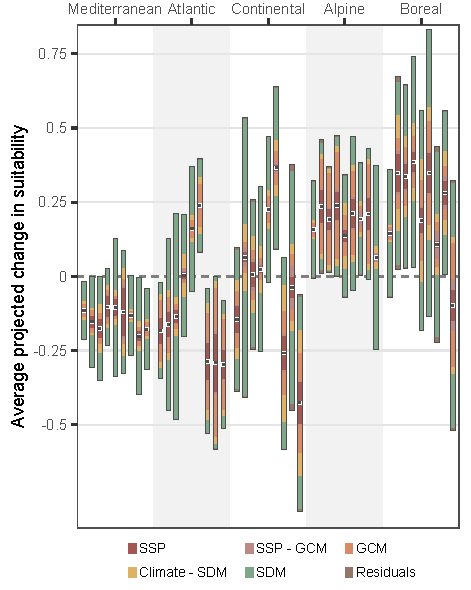
\includegraphics{figures/anova_within_species_byecoregion-1.pdf}
\caption{\textbf{Variance partitioning across Europe's ecoregions, for each species.} An ANOVA-based variance decomposition was performed to distinguish between 5 main uncertainty sources: (i) the future scenario (SSP), (ii) the climate model used to generate the climate projections (GCM), (iii) the interactions between the SPP and the GCM, (iv) the species distribution modeling method (SDM approach), and (v) the interactions between SDM approach and climate projections (both GCMs and SSPs). The black line represents the mean projection, across all GCMs, SSPs, SDMs and species. 90\% uncertainty ranges were calculated additively and symmetrically around the mean. Inset plot shows the species name in the same order than in the main plot.}
\label{fig:anovawithinspecies}
\end{SCfigure} 

Our results also revealed that the divergent projections between SDM approaches followed a regular pattern. 
At the European scale, CSDM projections projected systematically stronger decrease in climatic suitability for all species than expert PEMs, especially in Mediterranean and Atlantic ecoregions and in the western part of the Continental ecoregion (\Cref{fig:cascade,,app:qrobproj,,app:qpetproj,,app:qileproj,,app:qpubproj,,app:aalbproj}). Note the exception of holm oak for which the suitability decrease is more significant in the Mediterranean Basin according to PEM projections (though the average suitability across Europe remains more optimistic than other models, \Cref{app:qileproj}). Overall, expert PEMs also simulated a higher increase of suitability in the transition zone between Continental and Boreal ecosystems. Fitted PEMs  projections were closer to CSDM projections in the Southern and Western parts of Europe, i.e. the trailing edge of the range of most species, whereas they were closer to expert PEM ones in the North-West leading edge (\Cref{fig:cascade,,app:qrobproj,,app:qpetproj,,app:qileproj,,app:qpubproj,,app:aalbproj}). These discrepancies between modeling approaches can significantly change projected trends at the country level. In Germany for example, beech showed an average suitability decrease of $-0.04$ ($\pm0.09$) in 2090 when considering only CSDM and fitted PEMs, i.e. the two SDM approaches entirely calibrated with current species distribution data, whereas the expert PEM simulated a suitability increase ($0.39\pm0.15$). These discrepancies were also reflected in the simulated distribution for 2090 (\Cref{fig:fagus,,app:qrobdist,,app:qpetdist,,app:qiledist,,app:qpubdist,,app:aalbdist}). Beech did not show major extinction according to the expert PEM, whereas it was predicted to disappear from a large part of South-Western Europe by the CSDMs and the fitted PEMs (\Cref{fig:fagus}). Partially fitted PEM projections were generally closer to expert PEM ones (\Cref{fig:cascade}), but still simulate greater extinctions at the distribution limits of beech (\Cref{fig:fagus}).
Finally, disagreement between models within a model approach (area where less than 80\% simulations show same sign of suitability change) varied geographically. For example, for beech, PEM projections mostly  disagreed in Mediterranean and Atlantic ecoregions whereas CSDM simulations disagree in the eastern half of Europe (\Cref{fig:cascade}).

\begin{figure}
\centering
\hspace*{-2cm}
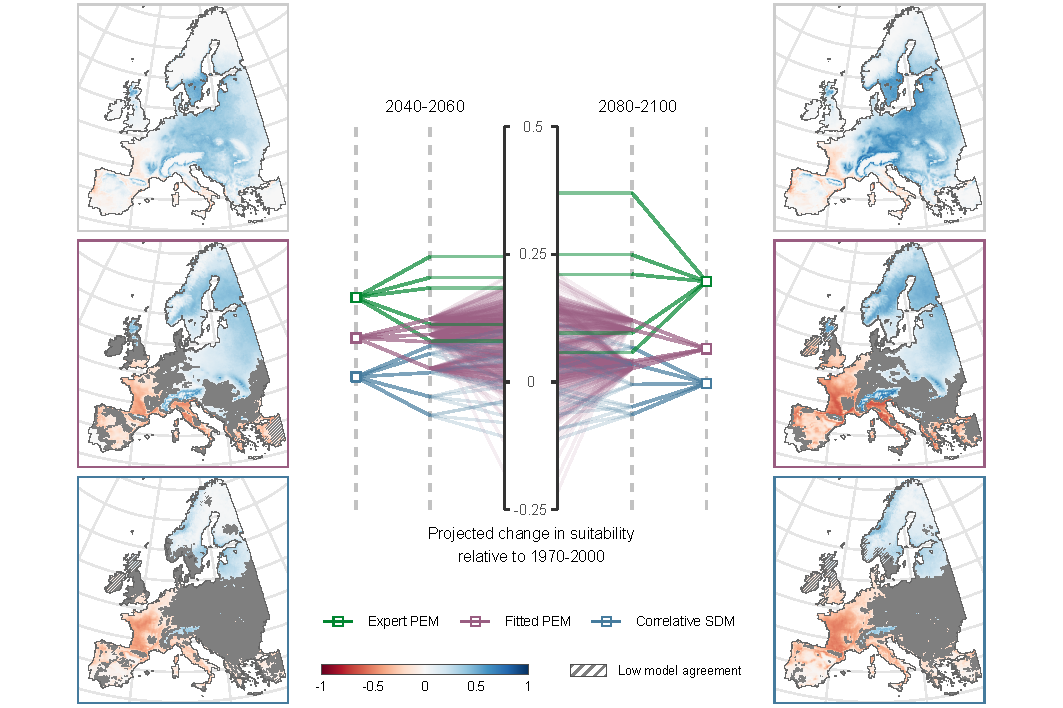
\includegraphics[width = 22cm]{figures/fagus_cascade-1.pdf}
\caption{\textbf{Discrepancies between model approaches in projected future climatic suitability change for beech.} Models are forced with climatic data from 5 GCMs under scenario SSP2-4.5. Areas with a lack of model agreement (less than 80\% of the individual calibrations agree on the sign of the change) are marked by hatching. Each individual calibrated model (i.e. 4 different CSDMs, 100 fitted PEM parameter sets, 10 partially fitted PEM parameter sets, and 1 expert PEM parameter set) was run with the 5 different GCM climatic variables (i.e. 20 CSDM projections, 500 fitted PEM projections, 50 part. fitted PEM projections, and 5 expert PEM projections). Then, they were averaged at the GCM-level within each SDM approach ("\emph{GCMs multi-calibration means}"), and further averaged into one ensemble per SDM approach.}
\label{fig:cascade}
\end{figure}

\subsection{Discussion}

% Total uncertainty in projected climatic suitability change showed a strong dependency on the different classes of model.
Differences between model approaches generated high uncertainty in projected climatic suitability change. 
Across species, in a large part of Europe (Atlantic, Continental and Boreal ecoregions), discrepancies between modeling approaches are a more important source of uncertainty than the differences among climate model projections (GCMs) and socioeconomic scenarios (SSPs). In the Boreal ecoregion -- where two very important forestry countries in terms of wood stock, added value, and forest-based workforce are located (Finland and Sweden) -- SDM approaches are even a higher source of uncertainty (33.7\% on average) than the difference across species (14.4\%). In such notable case, it thus seems more critical to encompass the full model diversity rather than the full species diversity to get a comprehensive assessment of the magnitude of climatic suitability change. Note, however, that the models agree on more suitable climatic conditions in this region by the end of the 21\textsuperscript{st} century (\Cref{fig:anova2090A}). At the species-level, the differences between modelling approaches is the main source of uncertainty for all the species considered here, and explain between 45\% and 60\% of the total uncertainty on average (\Cref{fig:anovawithinspecies}). 
One of the striking example is the climatic suitability change of sessile oak in the Atlantic region, where it represents an important cultural and economic value, and for which more than 80\% of the uncertainty in climate change impact projections was due to variations among the different approaches of SDMs.

Previous studies had already shown that uncertainties within correlative models can be important  \citep{Thuiller2019}. For example, in \citet{Wessely2024}, the proportion of species from the current European species pool that cannot be sustained throughout the century ranges from 24.5\% (GLM) to 76.6\% (Random Forest). Here we show that when considering a larger diversity of models, the total uncertainty in species climate suitability is even higher (\Cref{fig:anovawithinspecies,,app:anovawithinspeciesCSDM}). Note in addition that we considered only one process-explicit model and focused on diverse approaches along the correlative-process continuum, but differences between process-explicit models can also be higher than differences between climate projections \citep{Asseng2013}. Ignoring the full diversity of models bias the estimation of other effects. For example, for beech, we would have estimated that discrepancies between GCMs would have been the major source of uncertainties (39.8\%), higher than the SDM uncertainty (33.8\%), whereas it was in reality much lower (18.8\%) than SDM uncertainty (51.2\%) when considering the three approaches of SDMs. Ignoring a large portion of uncertainty in species range projections due to modelling approaches can thus lead to overly confident predictions about which species will or will not be able to survive in future climates.  This becomes increasingly true as we approach the end of the 21\textsuperscript{st} century, where larger climate changes result in larger variation among projections (\Cref{fig:anovaecoregions}).

\begin{figure}[t]
\hspace*{-2cm}
\begin{subcaptiongroup}
\phantomcaption\label{fig:fagusA} 
\phantomcaption\label{fig:fagusB}
\phantomcaption\label{fig:fagusC}
\end{subcaptiongroup}
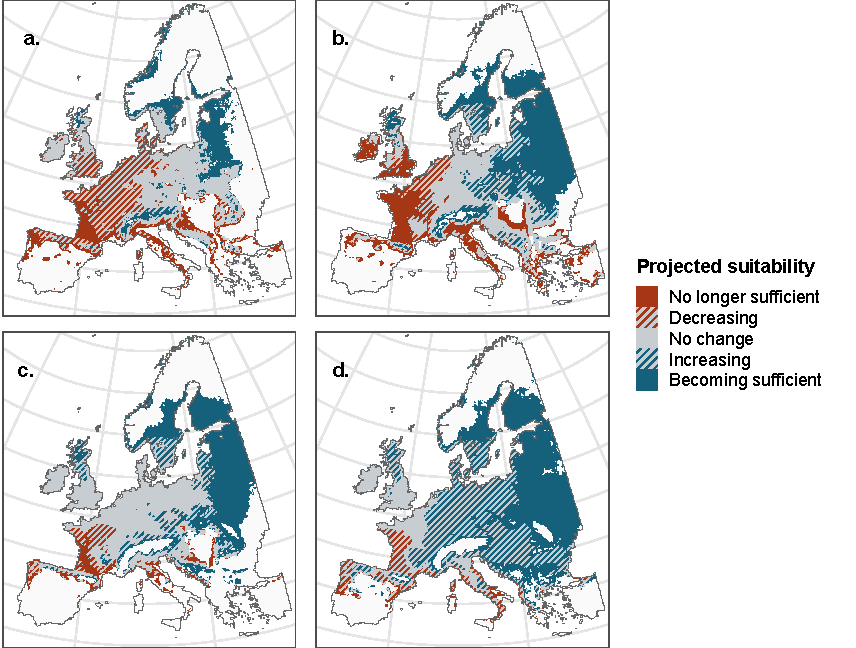
\includegraphics[width = 20cm]{figures/fagus_distributions-1.pdf}
\caption{\textbf{Projected beech distribution in 2090, according to (a) correlative species distribution models, (b) fitted process-explicit models, (c) partially fitted process-explicit models and (d) expert process-explicit models.} Models are forced with climatic data from 5 GCMs under scenario SSP2-4.5. For each model approach, the species is considered present/absent if more than half of the simulations agree.}
\label{fig:fagus}
\end{figure}

% What it implies in term of modeling bias // real climate threats?
CSDM and PEM future projections are known to diverge significantly \citep{Morin2009, Keenan2011a, Cheaib2012, Takolander2019}.
Here we show for the first time that the larger extinctions predicted in South-western Europe is associated to the method of calibration used. Indeed, the modeling approaches -- either statistical or process-explicit -- that were fit to current species distribution data predict greater extinctions at the southern edge of species ranges than expert PEMs (\Cref{fig:fagus}). Interestingly, we observed a gradient from correlative approaches fully determined by the current distribution to process-explicit approaches partially fitted with these data (\Cref{fig:cascade}). Although we cannot determine which approach truly overestimates or underestimates future climatic threats (but see \citealp{VanderMeersch2024}; \hyperref[chapter2]{Chapter 2}), we can hypothesize that distribution data are partly responsible for this pattern. This might be due to the fact that contemporary species occurrences are influenced by anthropogenic land use change which bias models calibration and may lead to smaller projected ranges \citep{Ay2017, Faurby2018}. This bias may be partly removed by including past occurrences data \citep{Faurby2018}, or by taking into account human-driven habitat modifications in the models \citep{Ay2017}. However, at the coarse scale of this study (0.1\degree), the bias may rather be due to the fact that recent distribution data do not cover the entire fundamental niche of the species, and thus that we underestimate the range of climatic conditions where species could survive \citep{NoguesBravo2016, Chevalier2024}. This fundamental niche truncation could be partly corrected by including paleorecords in the calibration process \citep{Maiorano2013}, but it may even increase the magnitude of projected future changes for some plants. For example, in \citet{NoguesBravo2016}, the genus \emph{Fagus} shifted from a conservation status of "\emph{Least Concerned}" to "\emph{Endangered}" by 2050 in Europe when including such very long-term data. Another lever for improvement could be to consider local adaptation potential of species \citep{BenitoGarzon2011}, as some populations may be pre-adapted to more challenging climatic conditions. In any case, including past distribution data or refining model with finer-scale data cannot prevent the issue of non-analogue future climatic conditions. Most paleorecords are limited to the Late Pleistocene/Holocene period (but see \citealp{Chiarenza2023}), i.e. to a cooler climate, and estimating the actual warm niche limits would require going back much further in time where paleorecords become even more challenging to use, and potentially where modern species did not yet exist \citep{Burke2018, Chevalier2024}. Process-explicit models are not concerned by bias in occurrence data when they are calibrated on experimental data -- even though it can be also challenging to represent future climatic conditions in experiments (particularly extreme temperatures) -- and may be more robust to novel climates (\citealp{VanderMeersch2024}; \hyperref[chapter2]{Chapter 2}). In addition to fewer projected extinctions, PEMs, either expert or fitted, also projected more substantial range expansions towards the North and the East of Europe for most species considered here (consistently with other taxa, \citealp{Buckley2010}). Therefore, interestingly, fitted PEMs exhibited an intermediate behavior between CSDMs and expert PEMs: they lead to both larger extinctions in the South-Western part of Europe like CSDM and to larger climatic suitability increases in the North and Eastern part like expert PEMs. The constraints imposed by the structure of process-explicit models during the calibration may explain why they differ from correlative models, even though mathematical functions alone do not sufficiently constrain the calibration process (\hyperref[chapter3]{Chapter 3}).

Beyond the differences between SDM approaches, multi-model projections are particularly useful for identifying general trends and guiding forest management. Such multi-model ensembles have been so far mostly restricted to statistical models \citep{Simmonds2024}, but we show here that there is a strong interest in considering a broader range of models to better characterize projections uncertainty. At the continental scale, it is possible to distinguish several regions that differ in terms of future climate risks and levers of action to address them (\Cref{fig:anova2090}). Around the Mediterranean Basin and in South-western France, the models agree in predicting generally less favorable climatic conditions for the species we considered here. In particular, the suitability of temperate broadleaf species (sessile and pedunculate oaks, beech) is projected to decrease while that of Mediterranean species (pubescent and evergreen oaks) is projected to increase. In some areas, evergreen oak has already replaced beech \citep{Penuelas2003}. However, process-explicit model projections are more nuanced for deciduous oaks and beech in France, suggesting that some better-adapted populations will survive if the existing standing genetic variation is maintained and promoted by forest managers \citep{Brang2014}. On the contrary, the Scandinavian and Baltic countries, part of Poland and low mountain ranges of Central-Eastern Europe (Carpats, Ore Mountains, Sudetes) are projected to get an overall increase of climatic suitability. Thanks to a more favourable climate and an extended growing season, beech has been shown to be already more competitive at the northern margin of its range \citep{Bolte2010}, and could be favoured to convert pure coniferous stands into mixed forest in order to increase their resilience \citep{Schauer2023}. Climatic suitability is also projected to increase in the Alps and in the Scandinavian Mountains, but these areas are subject to a greater uncertainty related to climate projections (\Cref{fig:anovaecoregions}), likely due to the more complex topography. 

Large zones of Europe though exhibit less clear trends. There is a notable low agreement among models in the Continental ecoregion, which includes some countries with important forest sector (Germany, Romania...), as well as in the British Isles (except Scotland). In those regions, species-related uncertainty plays a major role (\Cref{fig:anova2090A}) and indicates that one of the strategies to consider is the diversification of tree species, but also an increased genetic diversity within populations, to mitigate the risks associated with uncertain future conditions \citep{Morin2014, Ammer2019, Pretzsch2021, Vospernik2024}. Such unclear trends are also visible in the mountainous regions at the transition between Mediterranean and Continental/Atlantic climates (Pyrenees, Massif Central, Balkans). Finally, in some areas where most species are threatened, forest managers may consider introducing new species, more drought-tolerant. However, the lack of hindsight and experimental data often prevents the development and calibration of process-explicit models for such species.

We assessed uncertainties in species climatic suitability by quantifying the variance across the projections of a set of different models making the important hypothesis of equal likelihood of the projections of each model approach. As with climate models \citep{IPCC2021}, the spread in the projections could be reduced by weighting models according to their ability to reproduce past observations. A model’s credibility is indeed increased if the model is able to simulate past species range shifts, especially under climatic conditions that significantly differ from the present ones. The ability to reproduce changes in tree distributions during large paleoclimate fluctuations is known to vary across the different approaches of species distribution modeling (\citealp{VanderMeersch2024}; \hyperref[chapter2]{Chapter 2}). In particular, CSDMs showed less accurate predictions of species distribution change since the early Holocene (12,000 years ago) than process-explicit models (\citealp{VanderMeersch2024}; \hyperref[chapter2]{Chapter 2}). Previous studies also pointed out that CSDMS projections for the coming decades would decline steadily  in response to increasing climate novelty \citep{Fitzpatrick2018}. However, model evaluations using paleorecords may be biased by the sparse coverage in pollen data they used to infer past species distributions, and the magnitude and rate of future climate change will differ from the changes that occurred between the Last Glacial Maximum and today (the period for which most pollen records are available). 
It thus seem overly optimistic to summarize model discrepancies in one performance metric and then use it as the unique criteria in a model weighting scheme. Even when multivariate metrics are available, such as for climate models, there is no consensus that model weighting is more reliable than the "one-model-one-vote" strategy \citep{IPCC2021}.

Our results emphasise that it is critical to consider the diversity of modeling approaches that exist in order to ensure a consistent quantification of all model-related uncertainties in future species range shifts. Failure to fully quantify and report uncertainty, whether intentionally to preserve core messages, or not, leads to overconfidence in model projections \citep{Simmonds2024}, and may negatively impact public trust in scientists \citep{Howe2019}. To ensure the resilience and sustainability of Europe's forests, forest managers need to adopt adaptive management strategies that take account of all possible future conditions. 


\end{linenumbers}
\end{doublespacing}

%%%%%%%%%%%%%%%%%%%%%%%%%%%%%%%%%%%%%%%%%%%%%%%%%%%%%%%%%%%%%%%%%%%%%
%\section{Acknowledgments}
%%%%%%%%%%%%%%%%%%%%%%%%%%%%%%%%%%%%%%%%%%%%%%%%%%%%%%%%%%%%%%%%%%%%%
%\lipsum[13] 


%%%%%%%%%%%%%%%%%%%%%%%%%%%%%%%%%%%%%%%%%%%%%%%%%%%%%%%%%%%%%%%%%%%%%
%\section{Author Contributions}
%%%%%%%%%%%%%%%%%%%%%%%%%%%%%%%%%%%%%%%%%%%%%%%%%%%%%%%%%%%%%%%%%%%%%
%Conceptualization: Methodology: Investigation: Visualization: Writing:  Editing: Funding Acquisition: Supervision: . 

%\section{Author Competing Interests}
%\lipsum[14][2]

%%%%%%%%%%%%%%%%%%%%%%%%%%%%%%%%%%%%%%%%%%%%%%%%%%%%%%%%%%%%%%%%%%%%%

\renewcommand\refname{References}
%%%%%%%%%%%%%%%%%%%%%%%%%%%%%%%%%%%%%%%%%%%%%%%%%%%%%%%%%%%%%%%%%%%%%
\begin{footnotesize}
%\renewcommand{\bibnumfmt}[1]{#1.}
\bibliographystyle{spbasic.bst} % abbrvnat or unsrt
\textnormal{\bibliography{phd_bibliography}}
\end{footnotesize}
\newpage


%%%%%%%%%%%%%%%%%%%%%%%%%%%%%%%%%%%%%%%%%%%%%%%%%%%%%%%%%%%%%%%%%%%%%
% Tables
%%%%%%%%%%%%%%%%%%%%%%%%%%%%%%%%%%%%%%%%%%%%%%%%%%%%%%%%%%%%%%%%%%%%%

%\newpage
%\include{table.tex}

%%%%%%%%%%%%%%%%%%%%%%%%%%%%%%%%%%%%%%%%%%%%%%%%%%%%%%%%%%%%%%%%%%%%%
% Figures
%%%%%%%%%%%%%%%%%%%%%%%%%%%%%%%%%%%%%%%%%%%%%%%%%%%%%%%%%%%%%%%%%%%%%
%\include{figures.tex}

\end{document}